%=== CHAPTER THREE (3) ===
%=== (Actual work done and contribution, including literature survey) ===

\chapter{RVPG: Refined VP Guided Lane Detection}
\label{cha:model}
\begin{spacing}{1.5}
\setlength{\parskip}{0.3in}

\section{Introduction}

This chapter will describe the network structure of my work and how I implement it in both CAFFE and PyTorch. In \autoref{sec:MD_model}, I give the entire network an overview and explain the multi-task used in it. In \autoref{sec:MD_CAFFE}, I discuss the details of implementation in CAFFE, including data format, compiling environment, and the 4-Map VP feeding scheme. In \autoref{sec:MD_PyTorch}, I explain why PyTorch is better than CAFFE and how I implement the network in PyTorch. In \autoref{sec:MD_2D}, I describe the 2-D Gaussian algorithm, which is an improvement in utilizing the vanishing point.

\section{Improved Vanishing Point Directed Neural Network}
\label{sec:MD_model}

\subsection{Overview}
The network in my work is called \textbf{RVPG Net (Refined Vanishing Point Guided Network)}. It was developed based on the VPGNet~\cite{lee2017vpgnet} and had several improvements. The network aims at detecting and classify the lanes and the road markings simultaneously, on the pixel level. The lanes are predicted with on the guide of the vanishing point. 

Multi-task combined with Convolutional Neural Network is a solid solution in traffic-sign prediction. In research about traffic-sign design in 2016~\cite{zhu2016traffic, huval2015empirical}, researchers proposed a deep Convolutional Neural Network (CNN) structure to detect and classification those small-scaled road markings. Besides, they proposed a benchmark containing a variety of traffic signs and road markings. Because this network is good at small object detection, it can extract the high-level features from the image, thus, are more resistant to distortion in a small area. This stability can be extended to application in rainy conditions, that the rain drop's adverse effects will be offset. Based on their work, the RVPG net also uses the CNN structure and multi-task method to resist raindrop and lousy illumination distortion.

Vanishing points can direct the prediction of curved roads. The vanishing point is the visual intersection of two parallel lines. In our case, the vanishing point is the end of two converging lanes, as shown in TBC. Human eyes utilize this Vanishing Point information, usually unconsciously, to guess the curved road trend. By this mechanism, humans can predict a long-distance tendency rather than focus only on the short distance in front of the car.

The main feature of the RVPG is the multi-task and the VP feeding. With these two structure designs, the RVPG can extract the features from the original image significantly. It shows high accuracy \& F1-Score in the detection and classification of road markings.

\subsection{Architecture}

The architecture of the RVPG is shown in \autoref{fig:structure}. It mainly consists three stages:

\begin{enumerate} \vspace{-5mm}
    \item The convolution layers stack
    \item The multi-branch
    \item The feature combination layers stack
\end{enumerate} \vspace{-5mm}

\begin{figure}[ht]
\centering
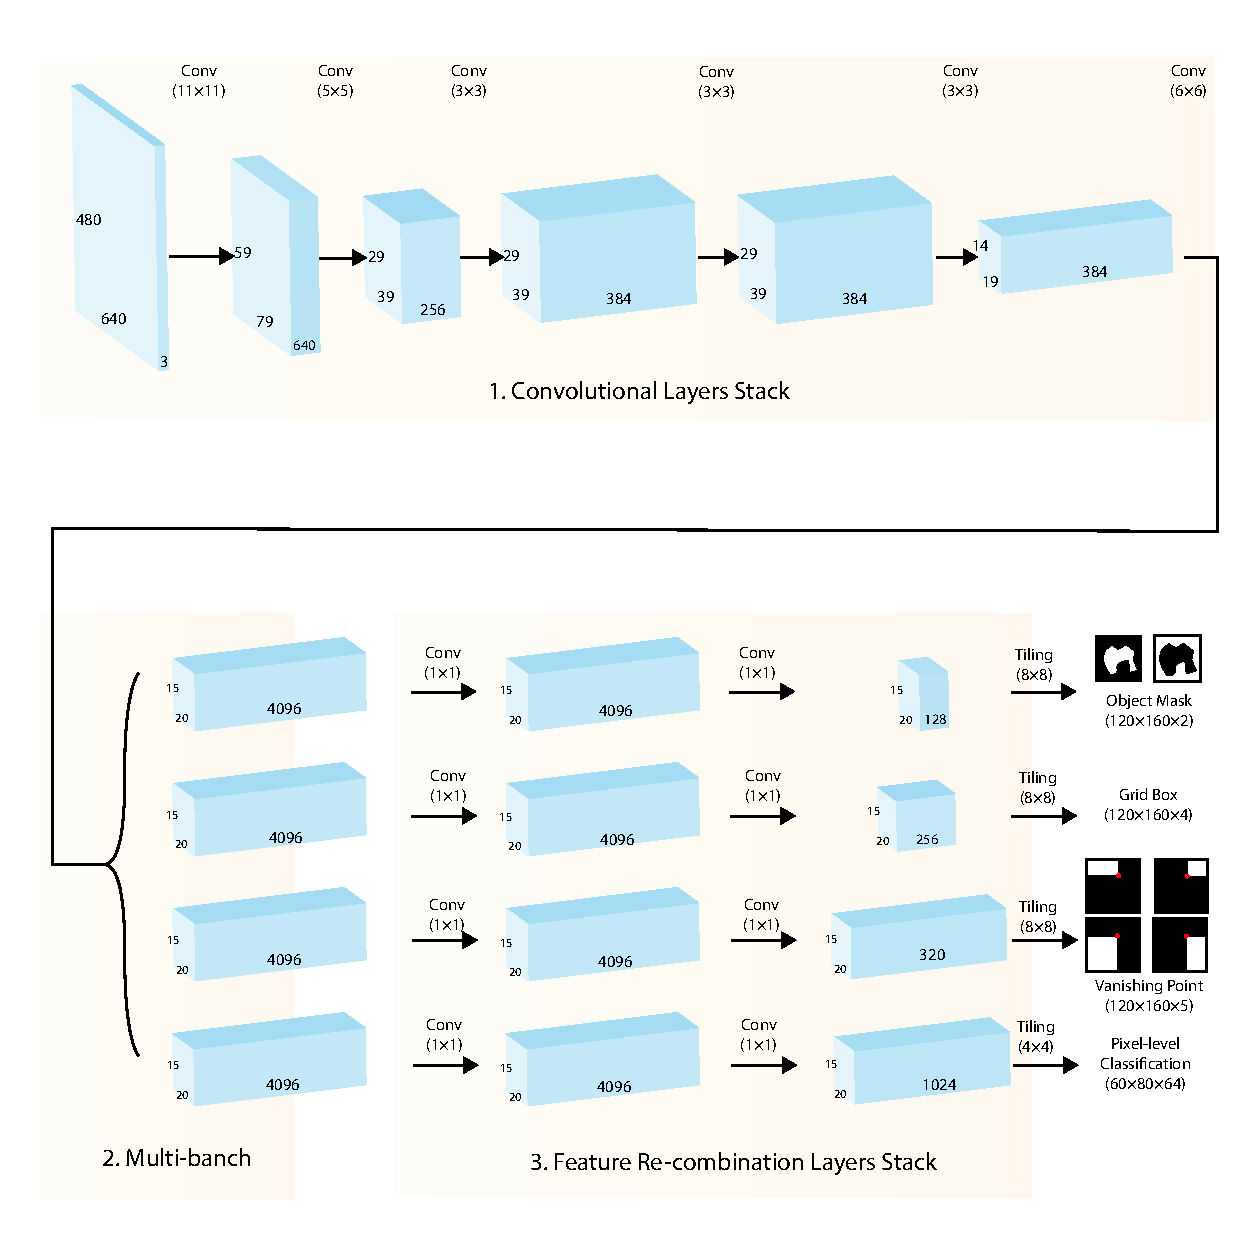
\includegraphics[width=0.99\textwidth, fbox]{Chapter3/structure.pdf}
\caption{the Structure of RVPG Network}
\label{fig:structure} 
\end{figure}

The first stage is a convolutional layer stack structure. It is aimed at extracting features. The input image is of size $480 \times 640 \times 3$\footnote{Because of the relatively fixed structure of the network, in RVPG, only 480*640 can be accepted as input. However, re-design on network convolutional layer configuration will fit any other size.}, $3$ is the RGB three-color channel. Like the CNN, the first stage of RVPG uses different $2-D$ convolutional kernel sizes to convolve the input image. In RSVP, we use the ReLU (Rectified Linear Unit, shown in \autoref{fig:relufunc}) activation function to do non-linear mapping in neutron and the max-pooling layer to reduce the feature maps size. The target of this first stage is to extract a higher dimension of feature maps. For example, the first convolution layers' output represents the existence of the continuous edges around the object; the second convolution layers' output represents the relative position between those extracted edge features; the third convolution layers' output represents the group information of edges that are non-intersected; and so on. With deeper the convolutional operation goes, the more abstract the feature extracted is. In RVPG, five continuous convolutional layers are used in the first stage.

The second stage is the multi-branch which will split the task into four different tasks simultaneously. All tasks would share the parameters behind the bifurcation, but the parameters after the bifurcation would belong to each task separately. This design of multi-task has two advantages: 1) Let the different tasks share information. 2) Do multi-task prediction. This structure will be explained in \autoref{subsec:multitask}.

The third stage is the feature re-combination layers stack, which aims to convergence feature map depth towards output size. This stage's structure is similar to CNN (As shown in the lower half of \autoref{fig:structure}), but with very thick feature map layers. As can be seen, the feature map depth is $15 \times 20 \times 4096$, $15 \times 20 \times 4096$ and $15 \times 20 \times k$, in which $k \in \{128, 256, 320, 1024\}$ for different branches. Each of the convolutional layers is using $1 \times 1$ convolutional kernel. Here, the $1 \times 1$ convolutional kernel is a way to reduce output dimension. As shown in \autoref{fig:oneonekernel}, if we want to reduce a feature map stack of size $W \times H \times N$, to $W \times H \times D, (D \neq N)$, just apply $D$ kernels of $1 \times 1 \times N$ size.

\begin{figure}[ht]
\centering
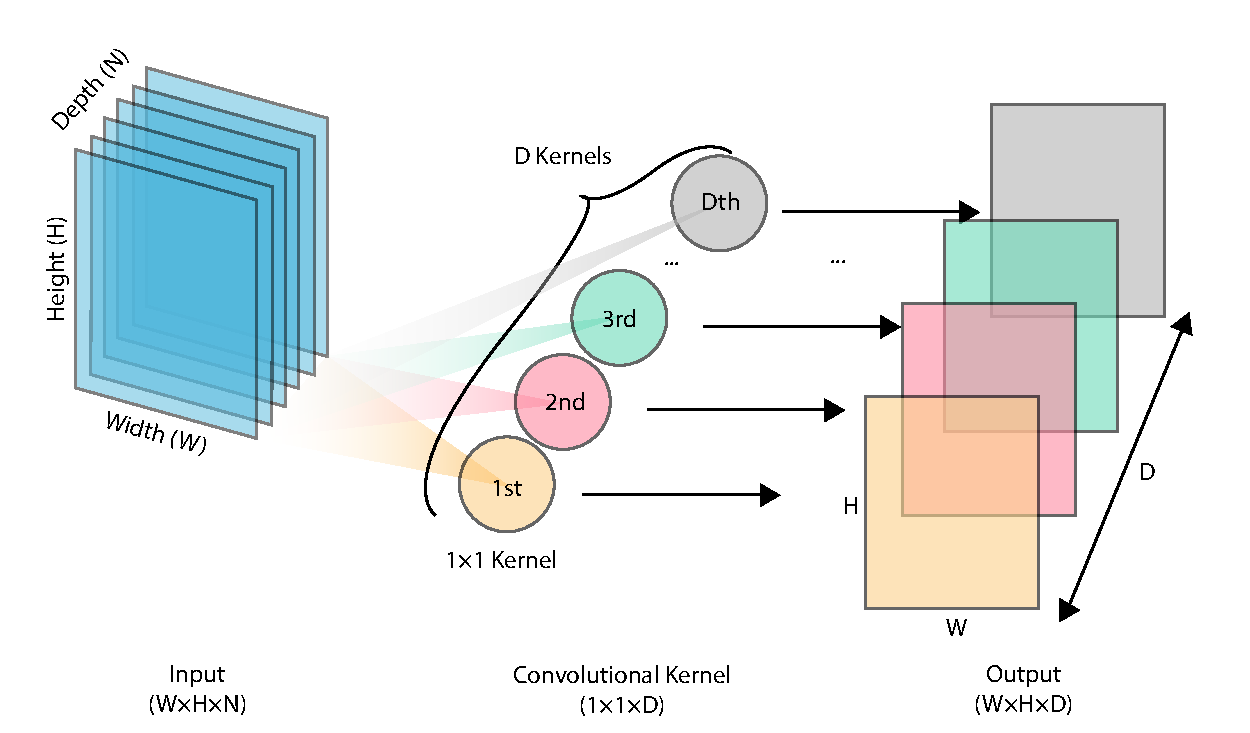
\includegraphics[width=0.99\textwidth, fbox]{Chapter3/oneonekernel.pdf}
\caption{Relationship between Size of Input, Kernel Num and Output}
\label{fig:oneonekernel} 
\end{figure}

The entire convolutional layers stack configuration and its index are shown in \autoref{tab:convlayer}.

\begin{table}[ht]
\centering
\caption{Convolutional Layers and Pooling Configuration}
\label{tab:convlayer}
\resizebox{\textwidth}{!}{%
\begin{tabular}{@{}ccccc@{}}
\toprule
Layer & (Kernel Size, Stride, Pad) & (Pooling Size, Stride) & Addition & Receptive Field \\ \midrule
Conv 1 & (11, 4, 0) & (3, 2) & LRN & 11 \\
Conv 2 & (5, 1, 2) & (3, 2) & LRN & 51 \\
Conv 3 & (3, 1, 1) & $-$ & $-$ & 99 \\
Conv 4 & (3, 1, 1) & $-$ & $-$ & 131 \\
Conv 5 & (3, 1, 1) & (3, 2) & $-$ & 163 \\
Conv 6 & (6, 1, 3) & $-$ & Dropout & 355 \\
Conv 7 & (1, 1, 0) & $-$ & Dropout & 355 \\
Conv 8 & (1, 1, 0) & $-$ & Branched & 355 \\ \bottomrule
\end{tabular}%
}
\end{table}

The combination of three stages can achieve four tasks at one prediction. Besides, for each branch, the information learned from other branches may help network to know the context of input images.

\subsection{Multi-task Structure}
\label{subsec:multitask}

Multi-task structure is the main highlight of the RVPG net. The training network are divided into four branches, each branch stands for one task in the lane and road marking, as shown in struacture diagram in \autoref{fig:structure}
% \vspace{-0mm}
\begin{align}
    F = \frac{P_{obj}}{H \times W} \times 100\% \label{eq:fore}
\end{align}
\vspace{-7mm}
\begin{equation}
    B = \frac{P_{bg}}{H \times W} \times 100\% \label{eq:bg}
\end{equation}

The first branch is the object mask task, basically a semantic detection of the target object. Its output is of size $120 \times 160 \times 2$, containing two feature maps. In the $1$st feature map, the foreground pixels (detected objects) are set as $1$, and other pixels are $0$. In the $2$nd feature map, the foreground pixels are set to be $0$, and the background is set to be $1$. This scheme is better than only using a $1$ frame for background/foreground because only detect the background or foreground may be unstable when either of them is not easy to detect. By using both foreground and background, results can be combined for post-processing. For example, if using all-background, when the object is tiny, the percentage of \autoref{eq:bg} will be large, and the network will tend to predict all the pixels as background to achieve lower loss. In this situation, the foreground frame is essential. Using a loss function like the $F_1$ score, even a tiny area in the foreground will effectively affect the result. Thus, the model will not converge at all-back or all-fore by combining the foreground and background two frames.

The second branch is the grid box branch, which is additional information for locating the objects, but finally proved useless. This branch is originated from VPGNet~\cite{lee2017vpgnet}. It just feeds low-definition grid boxes to the network. Hopefully, the network will learn to locate the object on a rough coordinate. The experimental results without this branch do not differ; thus, we remove it in RVPG.

The third branch is the Vanishing Point prediction task, in which the network will predict a $(X, Y)$ coordinate of Vanishing Point based on the given image. This branch will output $120 \times 160 \times 5$ feature map. It uses $5$ channels, as 1) the First channel is the VP foreground map; 2) Second channel has all pixels on the left upper corner to the Vanishing point as $1$ and other pixels $0$; 3) Third channel has all pixels on the right upper corner to the Vanishing point as $1$ and other pixels $0$; 4) Fourth channel has all pixels on the left lower corner to the Vanishing point as $1$ and other pixels $0$; 4) Fifth channel has all pixels on the right lower corner to the Vanishing point as $1$ and other pixels $0$. Details are described in \autoref{subsec:fourmap}

The fourth branch is the pixel-wise classification task. For each class, the network will give a confidential value of each pixel belonging to this class. The output size is $60 \times 80 \times 64$, in which $64$ means it can predict a maximum of $64$ types of road markings and lanes. In the RVPG, we use the VPG data set and Cordova data set, in which only $17$ of road markings (including lane type) types are annotated. The classes and their index are listed in \autoref{tab:classes}.

\section{Caffe Implementation}
\label{sec:MD_CAFFE}

As the original VPGNet author implements the network using CAFFE\footnote{\url{https://github.com/SeokjuLee/VPGNet}}, we also use CAFFE as my start point. But judge from the results, CAFFE is not suitable to conduct quick deep learning experiments, and I would recommend follower researchers not using CAFFE but start with PyTorch or Keras based on our code.


\subsection{Database and Extraction}

Two sets of labeled lane data are used: 1) Caltech~\cite{caltech} lanes database; 2) VPGNet~\cite{lee2017vpgnet} Lanes and road marking database. The data set size and group information is shown in \autoref{tab:dataset}. 

\begin{table}[ht]
\centering
\caption{Dataset Size and Number of Classes Contained}
\label{tab:dataset}
\begin{tabular}{@{}ccccc@{}}
\toprule
Dataset & Group & Numbers & Lanes & Roadmarkings \\ \midrule
Caltech-lanes & Cordova 1 & 250 & 3 & $-$ \\
 & Cordova 2 & 406 & 3 & $-$ \\
 & Washington 1 & 337 & 3 & $-$ \\
 & Washington 2 & 232 & 3 & $-$ \\
(Total) &  & 1225 &  &  \\
VPG database & Scene 1 & 13387 & 8 & 9 \\
 & Scene 2 & 3998 & 8 & 9 \\
 & Scene 3 & 818 & 8 & 9 \\
 & Scene 4 & 2633 & 8 & 9 \\
(Total) &  & 20836 &  &  \\ \bottomrule
\end{tabular}
\end{table}

\begin{figure}[ht]
\centering
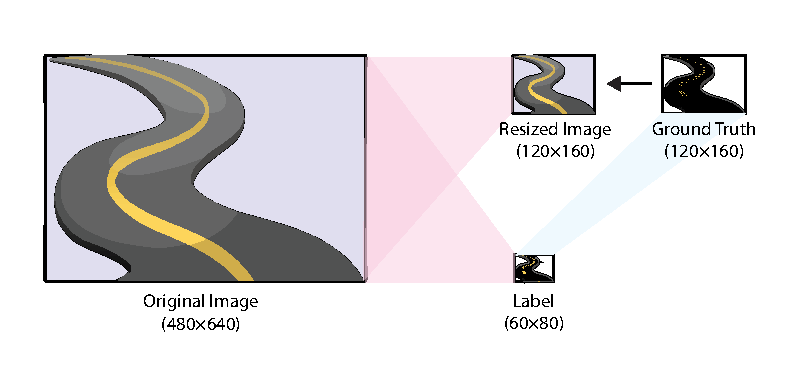
\includegraphics[width=0.99\textwidth, fbox]{Chapter3/gridbox.pdf}
\caption{Grid Box and Resize of Groundtruth}
\label{fig:gridbox} 
\end{figure}

First is the VPG data set, the mainly used data source in RVPG. It is recorded in Korean by Seokju Lee's team. In the VPG database, the image is not labeled pixel-wise but labeled with grids in size of $(8 \times 8)$ pixels. This is to comply with the network output size. As can be seen in \autoref{fig:structure}, Because the size of ground-truth is set to be $(120 \times 160)$ , each pixel in the ground-truth represents $4 \times 4 = 16$ pixels from the original $(480 \times 640)$ RGB-image ($480/120 = 4, 640/160 =  4$). So, although re-scaling the pixel-level annotation to $(8\times 8)$ pixels will lose some resolution, it is in fact not obvious in the $(120 \times 160)$ ground-truth, as shown in \autoref{fig:gridbox}. There are a total of $18$ classes used in VPG data, as shown in \autoref{tab:classes}. The $1$st class is for background, and the other $17$ classes are lanes and road markings. This data set's label is saved in \texttt{.mat} file in MATLAB matrix format.


\begin{table}[!ht]
\centering
\caption{Lane Classes in Caltech-lane Data Set}
\label{tab:caltech}
\begin{tabular}{@{}clcl@{}}
\toprule
Index & Lane Type & Index & Lane Type \\ \midrule
1 & Broken White & 4 & Broken Yellow \\
2 & Solid White & 5 & Solid Yellow \\
3 & Double Yellow & \multicolumn{1}{l}{} &  \\ \bottomrule
\end{tabular}
\end{table}


\begin{table}[ht]
\centering
\caption{Classes Specification in VPG and RVPG}
\label{tab:classes}
\begin{tabular}{clcl}
\toprule
Index & Lane Type          & Index & Road Marking Type   \\ \midrule
0     & Background         & 9     & Stop Line           \\
1     & Lane Solid White   & 10    & Arrow Left          \\
2     & Lane Broken White  & 11    & Arrow Right         \\
3     & Lane Double White  & 12    & Arrow Go Straight   \\
4     & Lane Solid Yellow  & 13    & Arrow U Turn        \\
5     & Lane Broken Yellow & 14    & Speed Bump          \\
6     & Lane Double Yellow & 15    & Cross Walk          \\
7     & Lane Broken Blue   & 16    & Safety Zone         \\
8     & Lane Slow          & 17    & Other Road Markings \\ \bottomrule
\end{tabular}
\end{table}%


Second is the Caltech-lanes Database, recorded with in-vehicle cameras in two cities: Cordova and Washington. Image from each city is divided into two groups, as shown in \autoref{tab:dataset}. It contains five classes of lanes only, and no road markings involved, as shown in \autoref{tab:caltech}

VPG data and Caltech data are saved in different formats. When they are fed into the RVPG network, they will be transformed to a CAFFE database format\footnote{the HDF5 format database and blob, as described in \url{https://caffe.berkeleyvision.org/tutorial}}. I provide the script in \autoref{apx:extraction}.

\subsection{Environment Configuration}

\begin{table}[ht]
\centering
\caption{Dependency Environment of CAFFE v1.0}
\label{tab:caffeenv}
\resizebox{\textwidth}{!}{%
\begin{tabular}{@{}llllll@{}}
\toprule
Package & Version & Build & Package & Version & Build \\ \midrule
CAFFE & 1.0 & $-$ & libprotobuf & 3.13.0.1 & hd408876\_0 \\
anaconda & 2020.07 & py38\_0 & mkl & 2020.1 & 217 \\
cryptography & 2.9.2 & py38h1ba5d50\_0 & numpy & 1.18.5 & py38ha1c710e\_0 \\
cudatoolkit & 11.0.221 & h6bb024c\_0 & CUDA & 11.1 & $-$ \\
h5py & 2.10.0 & py38h7918eee\_0 & CuDnn & 8.0.4.30-1 & amd64 \\
hdf5 & 1.10.4 & hb1b8bf9\_0 &  &  &  \\ \bottomrule
\end{tabular}%
}
\end{table}

The main trouble in using CAFFE is the environment compiling, so in case anyone wants to reproduce the experimental results in CAFFE, the compiling details are given in \autoref{tab:caffeenv}.

My hardware environment is: Google Cloud Platform\footnote{\url{https://cloud.google.com/gcp}} n1-standard-4 (4 vCPUs, 15GB memory), $1 \times$ NVIDIA Tesla P4 GPU.

\subsection{4-Map: Vanishing Point Feeding Scheme}
\label{subsec:fourmap}

\begin{figure}[ht]
\centering
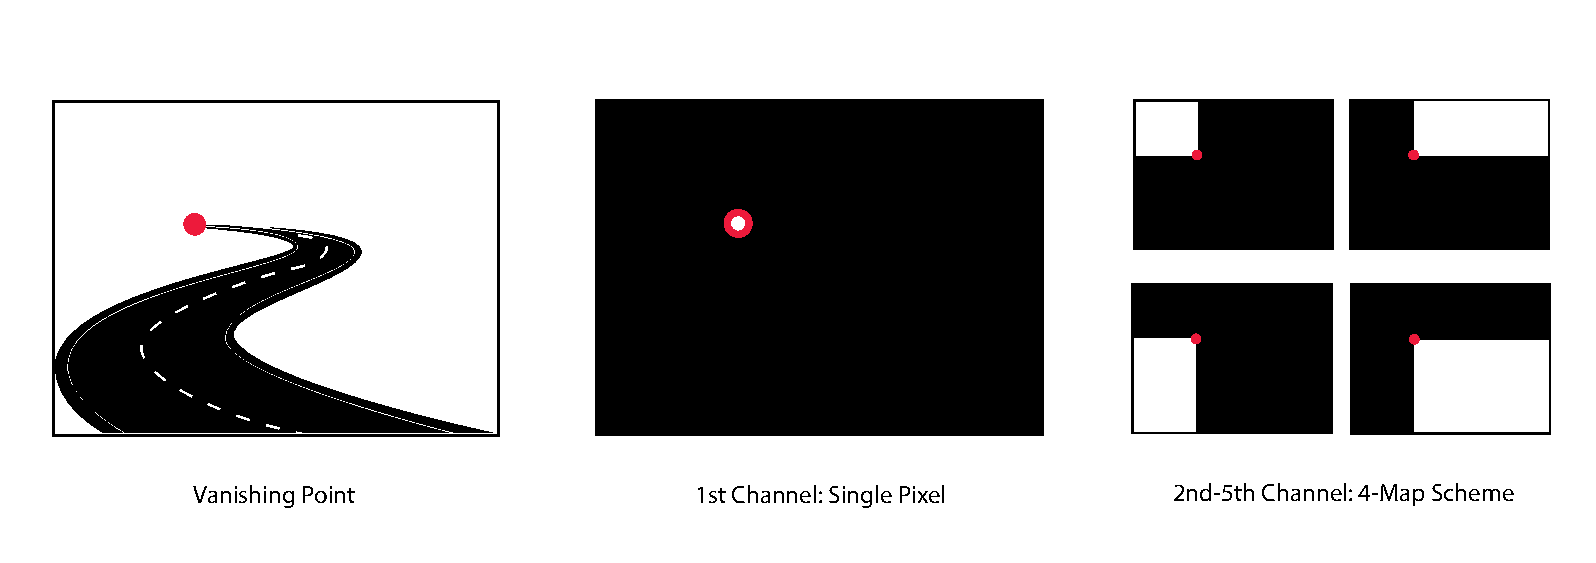
\includegraphics[width=0.99\textwidth, fbox]{Chapter3/fourmap.pdf}
\caption{4-Map Scheme in Vanishing Point Feeding}
\label{fig:fourmap} 
\end{figure}


Single point ground truth performs badly. When feeding the vanishing point information to the model (the  $3$rd branch in \autoref{fig:structure}), a single frame with a single vanishing point is difficult for the network to learn from. The vanishing point is just a single pixel on the feature map, occupying only $\frac{1}{640*480}$ percent. When fed into the network directly, the vanishing point is so small that the network would just ignore it and predict an all-background (no vanishing point exists). The network would reduce much more loss if work on other paths, so according to the rule of backpropagation (\autoref{subsec:back_propagation}), the network will just ignore this branch until it can put down loss anymore on other branches.

In RVPG, a 4-map scheme is being proposed. The intuition is that rather than a single pixel, a 4-map design would provide more information to the network. The ground truth used to training the network would be five channels. The first channel is still the single-pixel frame. The other four channels represent four corners of the vanishing point, as shown in \autoref{fig:fourmap}

This 4-map scheme can avoid the single-point dilemma. The network is provided with much more information about the relative position of the vanishing point in four directions. If just ignore or predict wrongly, the network will be punished by loss function severely. Thus, The network will converge on this branch.

\section{PyTorch Implementation}
\label{sec:MD_PyTorch}

\subsection{Motivation}

After implementation on the CAFFE, we move on to the PyTorch\footnote{\url{https://github.com/PrabhuSM16/VPGNet-Pytorch}}, a better place to conduct experiments. There are many four drawbacks in CAFFE: 

\begin{enumerate}

    \item CAFFE needs C++ debugging, which takes a long time to compile every time. As a large network like VPGNet, it usually takes more than $10$ mins per compilation.

    \item CAFFE is not friendly in document support and lacks the user-friendly API. Thus you need to go into all the C++ underlying code before making any change, even the most basic layer definition change. 

    \item CAFFE's support of GPU and CUDA suite is out-of-date, thus sometimes, with the newest computer with RTX 3080 GPU, you may even not able to call the GPU support with CAFFE. 

    \item The last but the most important, the whole community is moving on to the PyTorch and leave CAFFE back now. So code work in CAFFE will not be further used by any other researchers.
    
\end{enumerate}

\subsection{Data Format Conversion}

In PyTorch, we transform the data into the format that is applicable to Torch tensors\footnote{Tensors are data vectors flowing in PyTorch graph during training. It is defined by PyTorch.} and Numpy\footnote{Numpy is a common matrix calculation package in Python.}. 

PyTorch uses pixel-wise annotation. Because the labels can be read directly from \texttt{.mat} and \texttt{.ccvl} files to Numpy, there is no need to do an $8 \times 8$ grid scheme. In PyTorch, all the pixels are given an annotation without re-scaling or estimation. As a consequence, the model trained in PyTorch should be more precise than the one trained in CAFFE.

The code of this conversion function is given in \autoref{apx:pytorchdataloader}.

\subsection{4-Tilling: Redesigned Tilling Layer}

\begin{figure}[ht]
\centering
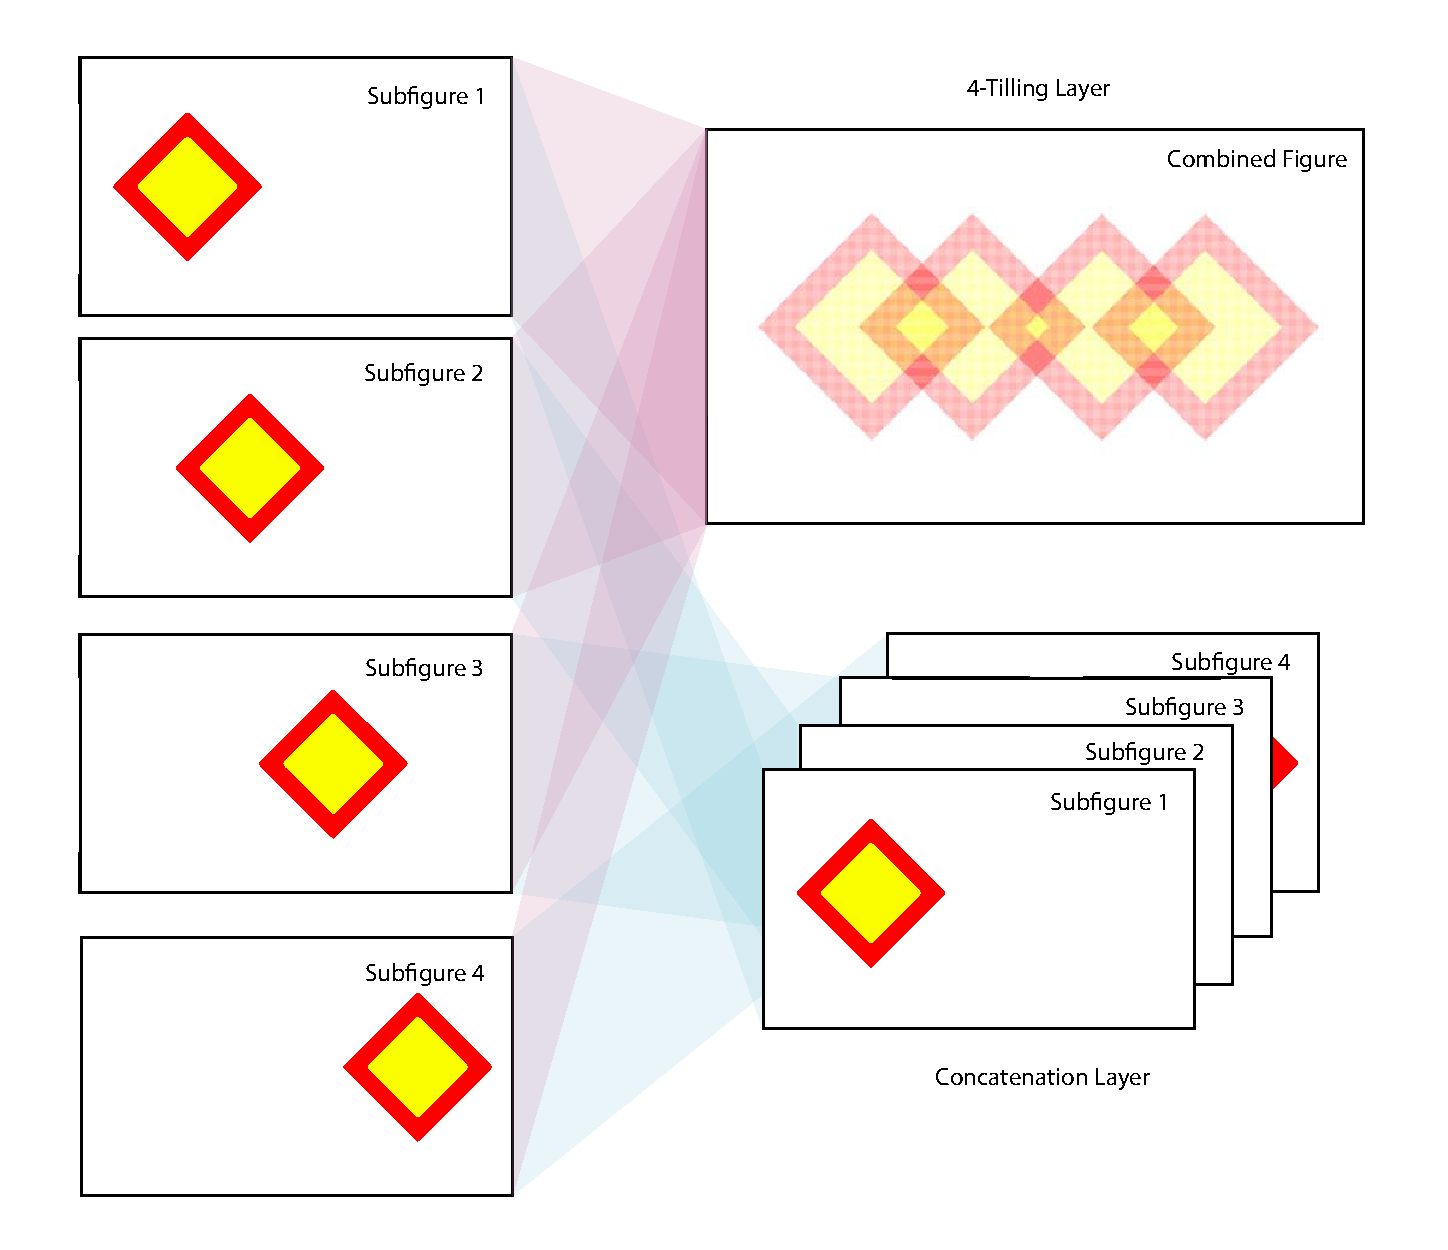
\includegraphics[width=0.99\textwidth, fbox]{Chapter3/fourtiling.pdf}
\caption{4-Tiling Combination V.S. Concatenate}
\label{fig:fourtiling} 
\end{figure}

In the RVPG, a re-designed combination layer called 4-tiling is proposed and implemented, and it has some advantages over the traditional concatenation layer, as shown in \autoref{fig:fourtiling}.

The traditional concatenation layer has some drawbacks. It simply concatenate $N$ numbers of $(W \times H)$ figures into a $(W \times H \times N)$ stack. If people want to reduce the depth of the output feature maps, it has to be passed through a convolutional kernel of size $(1 \times 1 \times N)$. The convolutional kernel will result in more computational resources be allocated.

To reduce the computational consumption, a 4-Tiling layer is designed. 4-Tiling is like aliasing and diffusion for four different sub-figures. The main advantage of 4-Tiling is not increasing the depth of the stack. After the 4-tiling, four $(W \times H)$ sub-figures are combined into one $(W \times H)$ figure. Compared with the concatenation layer, the 4-tiling layer doesn't need to use a convolutional kernel to reduce the output depth; thus, it is computation-economical.

As a result, using the 4-Tiling layer can reduce the computational resources needed by $N$ times.

\section{2-D Gaussian for VP Feeding}
\label{sec:MD_2D}

A better way to feed the vanishing point information to the network is the $2-D$ Gaussian. The formula of $1-D$ Gaussian is shown in \autoref{eq:1dgaussian}, in which $a,b,c \neq 0$ are constants.

\begin{equation}
\label{eq:1dgaussian}
    f(x)=\frac{1}{\sigma \sqrt{2 \pi }} \cdot e^{-\frac{(x- \mu )^2}{2 \sigma^2}}
\end{equation}

The 2-D Gaussian is like conduct Gaussian distribution both on $X$-axis and $Y$-axis. Its formula is shown in \autoref{eq:2dgaussian}. Its plot is shown in \autoref{fig:2dgaussian}.

\begin{equation}
\label{eq:2dgaussian}
    f(x,y)= A \cdot e^{-\left(\frac{(x- \mu_x )^2}{2 \sigma_{X}^{2}}+\frac{(y- \mu_y )^2}{2 \sigma_{Y}^{2}}\right)}
\end{equation}

\begin{figure}[!ht]
\begin{adjustbox}{minipage=0.98\linewidth,fbox}
    \centering
    \begin{subfigure}[b]{0.49\textwidth}
        \centering
        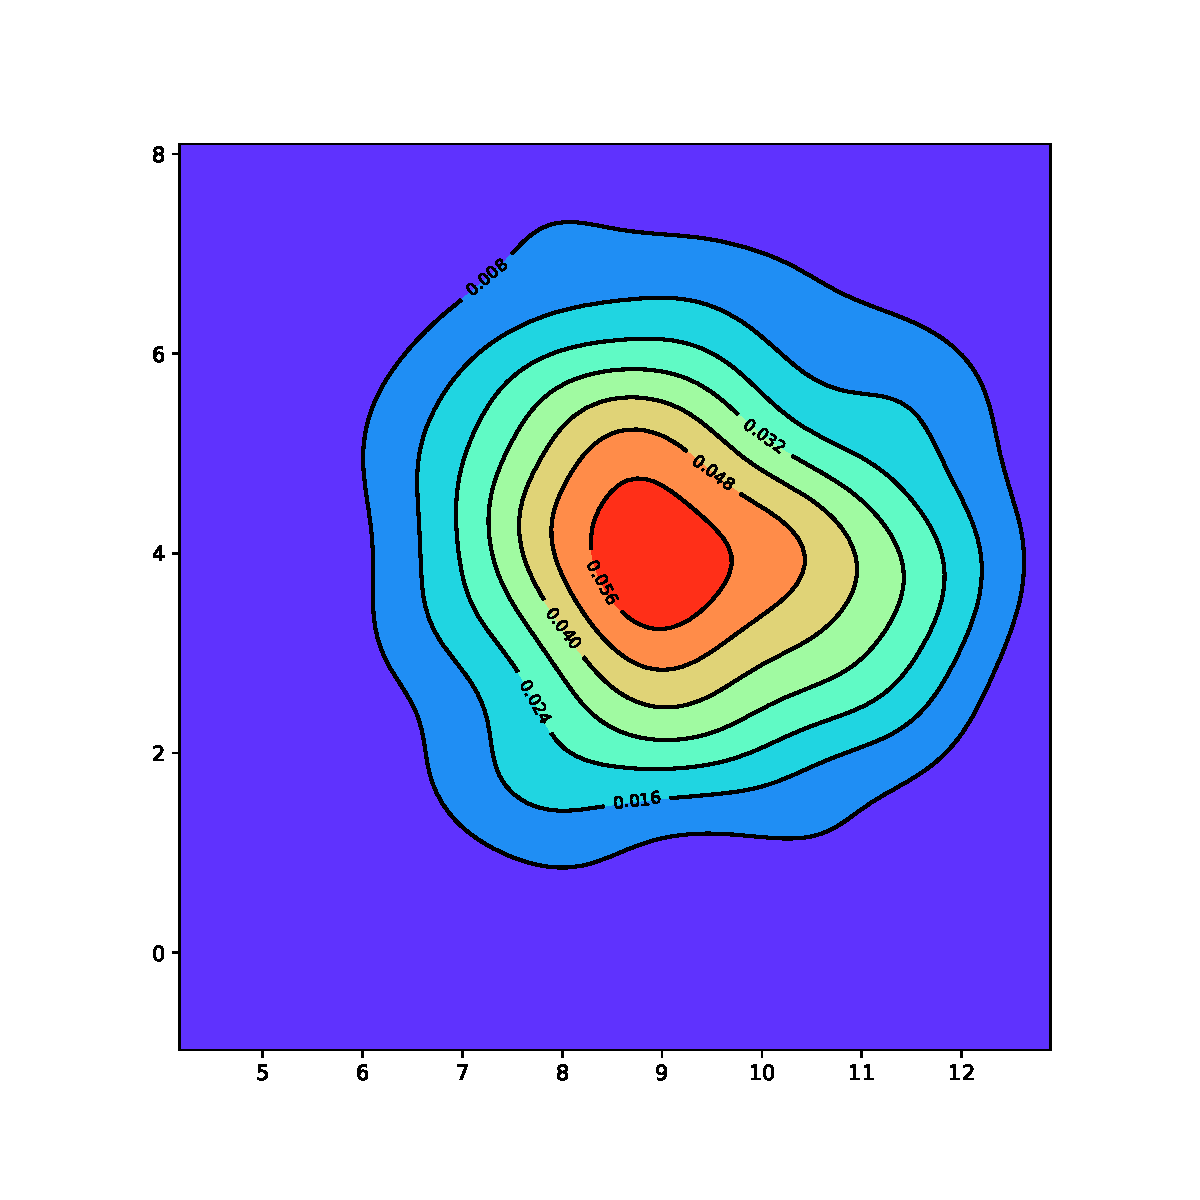
\includegraphics[height=2.3in]{Chapter3/gaussian2d.pdf}
    \end{subfigure}%
    ~
    \begin{subfigure}[b]{0.49\textwidth}
        \centering
        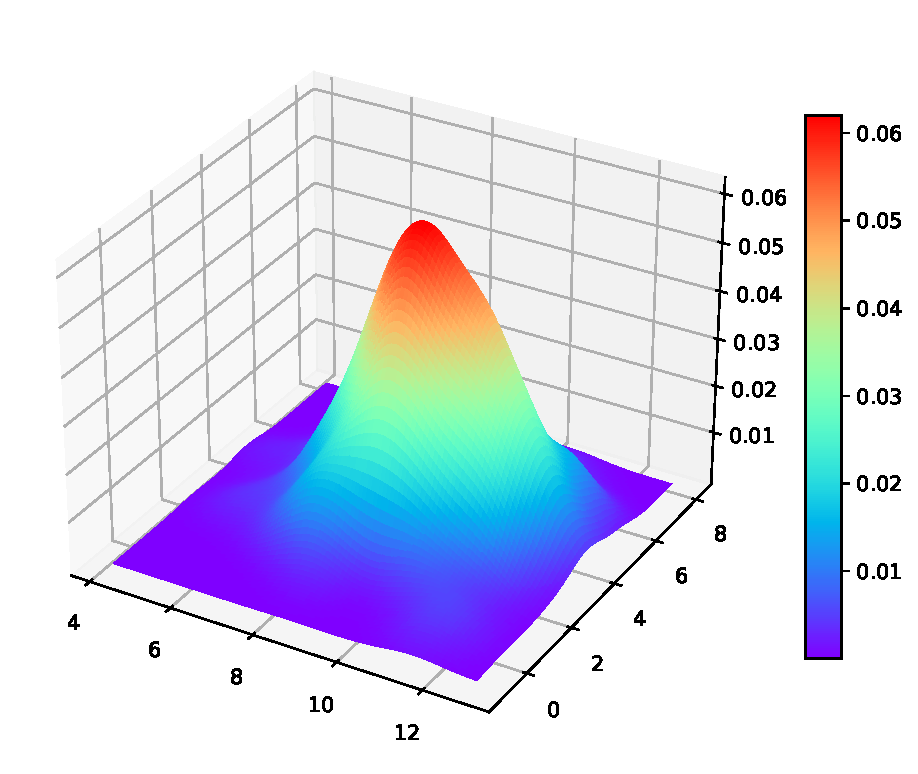
\includegraphics[height=2.3in]{Chapter3/gaussian3d.pdf}
    \end{subfigure}
\end{adjustbox}
\caption{2-D Gaussian Example}
\label{fig:2dgaussian}
\end{figure}

We can set the mean value $(\mu_x,\mu_y)$ as the vanishing point coordinate $(x,y)$, and the variance $(\sigma_X,\sigma_Y)$ differ according to the viewpoint of the in-vehicle camera. Compared to the single frame or 4-Map scheme, the 2-D Gaussian can provide more context to the network; thus, the VP information is expected to be learned better\footnote{2-D Gaussian is currently constructed with Numpy. Source code available on GitHub \url{https://github.com/PrabhuSM16/VPGNet-Pytorch}.}.

\section{Concluding Remarks}

In this chapter, I described the detail of the network structure of RVPG. I talked about how multi-task makes the network efficient and why the vanishing point is hard to learn in nature. I also give the details of CAFFE and PyTorch implementation.

Besides, three user-defined layers are described: the 4-Map, the 4-Tiling, and the 2-D Gaussian layers. They are not common deep-learning layers but designed and implemented especially for this network. They make the network grab information more efficiently.

In the next chapter, I will analyze the experimental results and some tools developed by me in experiments.

%=== END OF CHAPTER THREE ===
\end{spacing}
\newpage
